\chapter{Self-testing two-qubit maximally entangled states}
\label{chap:selftesting}

In this chapter we discuss the self-test of two-qubit maximally entangled states in a fully device-independent scope.
Specifically, we here present an ideal self-testing protocol based on correlations leading to a maximal \acrshort{chsh} score, i.e. the certification is solely based on that CHSH score.

\medbreak 

We consider the \acrshort{chsh} game in the quantum framework, where Alice and Bob receive copies of an unknown state $\rho_{AB} \in \mathcal{L}(\mathscr{H}^A \otimes \mathscr{H}^B)$ from an unknown source.
Alice has access to the subsytem that lays in the Hilbert space $\mathscr{H}^A$ while Bob has access to the one in $\mathscr{H}^B$, both of unknown dimension.
Each party has a measurement device with two inputs, $x,y=\{0,1\}$, respectively corresponding to observables $A_x$ acting on $\mathscr{H}^A$, for Alice, and $B_y$ on $\mathscr{H}^B$, for Bob.
These measurements only have two possible outcomes $(a,b)=\pm1$.
For each copies of the unknown share state, Alice and Bob randomly select a measurement and record that measurement outcome. 
This allows Alice and Bob to learn the statistics $p(ab|xy)$, from which can be computed the correlators $\mean{A_x B_y} = p(a=b|xy)-p(a\neq b| xy)$ and the CHSH score $S$ following \refeq{CHSH}. 
We here focus on the ideal-case where the maximal CHSH score is obtained, $S=2\sqrt{2}$ and from which we want to deduce the characteristics of the quantum realization $\{\rho_{AB},A_x,B_y\}$.

\medbreak

Let us first show that $A_x$ and $B_y$ fully specify the quantum model of the measurements.
As the measurements we consider have two outcomes $\{\pm1\}$, the quantum model of each observable is a \acrfull{povm} with two elements $\{M^{+1},M^{-1}\}$. We label $\{M_x^{+1},M_x^{-1}\}$ the POVM of $A_x$ and $\{M_y^{+1},M_y^{-1}\}$ the one of $B_y$.
Elements of these POVM satisfy
\begin{itemize}
	\item Hermitianity, $(M^{\pm1})^\dag=M^{\pm1}$,
	\item Positivity, $M^{\pm1} \succeq 0$, that is $\bra{\psi}M^{\pm1}\ket{\psi}$ for all $\psi$,
	\item Completeness, $M^{+1}+M^{-1}=\id$.
\end{itemize}
Alice and Bob's observables can be directly constructed from their respective POVM following
\begin{equation}
	\begin{split}
		A_x &= \sum_a \,a M^a_x = M^{+1}_x - M^{-1}_x, \\
		B_y &= \sum_b \,b M^b_y = M^{+1}_y - M^{-1}_y.
	\end{split}	
	\label{eq:obs_povm}
\end{equation}
%From this construction, we deduce that Alice and Bob's observables are Hermitian
%\begin{equation}
%	(M^{+1} - M^{-1})^\dag = (M^{+1})^\dag - (M^{-1})^\dag = M^{+1} - M^{-1},
%	\label{eq:obs_hermitian}
%\end{equation}
%and unitary
%\begin{equation}
%	(M^{+1}- M^{-1})^2 = (M^{+1})^2 - 2 M^{+1} M^{-1} + (M^{-1})^2 = M^{+1} + M^{-1} = \id.
%	\label{eq:unitary}
%\end{equation}
Using \refeq{obs_povm} and completeness, we can also show that each POVM element is fully described by the operator they correspond to, following
\begin{equation}
	\begin{split}
		M^{+1}_A = \frac{1}{2}(\id+A_x),\qquad & M^{-1}_A = \frac{1}{2}(\id-A_x) \\
		M^{+1}_B = \frac{1}{2}(\id+B_y),\qquad & M^{-1}_B = \frac{1}{2}(\id-B_y).
	\end{split}
\end{equation}

\medbreak
	
From the violation of the CHSH inequality, the first property of the quantum model we can deduce is that $\rho_{AB}$ is entangled.
Indeed, if the shared state is separable, then there exists weights $p_\lambda\geq 0$ and system states $\{\rho_{A}^\lambda\}$ and $\{\rho_{B}^\lambda\}$ such that
\begin{equation}
	\rho_{AB}^\text{sep} = \sum_\lambda\, p_\lambda\, \rho_{A}^\lambda \rho_B^\lambda.
\end{equation}
Therefore, the statistics $p(ab|xy)$ can be obtained by a local strategy where Alice and Bob's measurement devices first prepare the state $\rho_A^\lambda$ and $\rho_B^\lambda$, respectively, from the random variable $\lambda$, distributed according to $p_\lambda$, before measuring it according to $M^a_x,M_b^y$. 
Formally, that is
\begin{equation}
	\begin{split}
		p(ab|xy) &= \trr{\left(M^a_x \otimes M^b_y \right) \rho_{AB}^\text{sep}}  \\
				 & = \sum_\lambda\, p_\lambda \, \trr{\left(M^a_x \otimes M^b_y \right)\left(\rho_{A}^\lambda \otimes \rho_B^\lambda\right)} \\
				 & = \sum_\lambda\, p_\lambda\, \trr{M^a_x \rho_A^\lambda} \trr{M^b_x \rho_B^\lambda} \\
				 & = \sum_\lambda\, p_\lambda\, p(a|x,\lambda) p(b|y,\lambda).
	\end{split}
\end{equation}
From these statistics, a maximum CHSH score of $S=2$ can be expected.
Hence, a CHSH score $S>2$ rules out the possibility that the measured state is separable.

\medbreak

Another aspect we can deduce from a CHSH score $S>2$ is that the measurements are locally incompatible, i.e. $[A_0,A_1] \neq 0$ and $[B_0,B_1] \neq 0$.
To demonstrate this, let us focus on Alice's observables. 
If her measurements commute, then there would exist a basis $\{\ket{k}\}$, with $\ket{k}\in \Hil_A$, where both operators are diagonal and in particular
\begin{equation}
	\begin{split}
		A_x = \sum_k \ketbra{k} A_x \ketbra{k}.
	\end{split}	
\end{equation}
Using this basis, we construct an entanglement breaking quantum channel $\Lambda_A$ projecting the received state in Alice's local basis $\{k\}$ and discarding the measurement results. 
Formally, this channel acts on $\rho_{AB}$ as follows
\begin{equation}
	\begin{split}
		\Lambda_A[\rho_{AB}] &= \sum_k \left(\ketbra{k}_A \otimes \id_B \right)\rho_{AB}	\left(\ketbra{k}_A \otimes \id_B \right) \\
							 &= \sum_k p_k \ketbra{k}_A \otimes \rho_B^{(k)} \\
							 &= \tilde{\rho}_{AB} 
	\end{split}
\end{equation}
where $p_k$ is the probability to project $\rho_{AB}$ on $\ket{k}$.
Let us now compute the correlators appearing in the CHSH score on the state $\tilde{\rho}_{AB}$
\begin{equation}
	\begin{split}
		\mean{A_x B_y}_{\tilde{\rho}_{AB}} &= \trr{\tilde{\rho}_{AB}(A_x \otimes B_y)} \\
										   &=\trr{\sum_k \left(\ketbra{k}_A \otimes \id_B \right)\rho_{AB}	\left(\ketbra{k}_A \otimes \id_B \right) \left(A_x \otimes B_y\right) } \\
					   &= \trr{\rho_{AB} \sum_k \left(\ketbra{k}_A \otimes \id_B \right)\left(A_x \otimes B_y\right)\left(\ketbra{k}_A \otimes \id_B \right)  } \\	
					   &= \trr{\rho_{AB}\left(\sum_k \ketbra{k}A_x \ketbra{k}\right) \otimes B_y} \\
					   &= \trr{\rho_{AB}\left(A_x \otimes B_y\right)}.
	\end{split}
	\label{eq:compatible_separable}
\end{equation}
This shows the equivalence between correlations computed using locally compatible measurements and correlation computed using a separable state.
Therefore, a violation of the CHSH inequality, only possible for entangled states, is a proof of locally anticommuting measurements.

\medbreak

If entanglement and locally incompatible measurement are solely deduced from a CHSH score $S>2$, there is, however, more to deduce from a maximal CHSH score $S=2\sqrt{2}$.
More specifically, a maximal CHSH violation can only be achieved by a specific quantum model of a maximally entangled state and some locally maximally incompatible measurements, i.e. measurement with a zero joint measurability region~\cite{Summers1987,Popescu92,Tsirelson1993}.
Therefore, a maximal CHSH violation is a good criterion for a self-testing statement.

To formulate this statement, we first define the relevant Hilbert spaces.
We start by introducing $\Hil_{AB}= \Hil_A \otimes \Hil_B$, the basis in which the shared state is diagonal
\begin{equation}
	\rho_{AB} = \sum_i p_i \ketbra{\psi_i}	.
\end{equation}
As the observed statistics only depends on the support of $\rho_{AB}$, i.e. the states $\{\ket{\psi_i}\}$ for which $p_i\neq0$, we define the relevant space
\begin{equation}
	\Hil_{AB}^\star = \spn{\ket{\psi_i}\, | \, p_i \neq 0}.
\end{equation}
Similarly, we construct the relevant space for each parties' subsytem as
\begin{equation}
	\begin{split}
		\Hil _A^\star &= \spn{\ket{\psi_i}_A\, | \, p_i \neq 0} \\
		\Hil _B^\star &= \spn{\ket{\psi_i}_B\, | \, p_i \neq 0}.
	\end{split}
\end{equation}

Since the observables we consider have eigenvalues $\pm 1$, we can deduce the useful relation
\begin{equation}
	A_0^2 \ket{\psi}_A = A_1^2 \ket{\psi}_A = \ket{\psi}_A.
	\label{eq:involutory}
\end{equation}

Then, we recall the expression of the CHSH operator
\begin{equation}
	\mathcal{B}_{\mathrm{CHSH}} = A_0 \otimes \left( B_0 + B_1 \right) + A_1 \otimes \left( B_0 - B_1 \right)
\end{equation}
which is Hermitian by construction.
From the sum-of-square decomposition of the CHSH operator $2\sqrt{2}\id_{AB} - \mathcal{B}_\text{CHSH}$ we can show that
\begin{equation}
	A_0 A_1 \ket{\psi}_A = -A_1 A_0 \ket{\psi}_A 
	\label{eq:anticom}
\end{equation}
for all state $\ket{\psi}_A \in \Hil_A^\star$~\cite{Pironio2010,Supic2019}.

We label $\ket{0_k} \in \Hil_A^\star$ any eigenstates of $A_0$ satisfying $A_0 \ket{0_k} = \ket{0_k} $.
We then introduce $\ket{1_k} = A_1 \ket{0_k}$.
From \refeq{involutory} and \refeq{anticom}, we can check that the basis $\{\ket{0_k},\ket{1_k}\}$ is an orthonormal basis for which
\begin{equation}
	\begin{split}
		A_0 \ket{0_k} = \ket{0_k} \qquad & A_0 \ket{1_k} = -\ket{1_k} \\
		A_1 \ket{0_k} = \ket{1_k} \qquad & A_1 \ket{1_k} = \ket{0_k}.
	\end{split}
\end{equation}
Therefore, on the two-dimensional subspace spanned by $\ket{0_k},\ket{1_k}$, the operator $A_0$ and $A_1$ act as the Pauli operators $\sigma_z$ and $\sigma_x$, respectively. 
Repeating this process for all $k$ eigenvectors, we can write Alice's observables as a block-diagonal matrix with block of size $2 \times 2$
\begin{equation}
	A_0 = \bigoplus_k \sigma_z^{(k)}, \qquad A_1 = \bigoplus_k \sigma_x^{(k)}.
\end{equation}
Following the same steps for Bob, we find that his observables have the same block diagonal structure
\begin{equation}
	B_0 = \bigoplus_l \frac{\sigma_z^{(l)}+\sigma_x^{(l)}}{\sqrt{2}}, \qquad B_1 = \bigoplus_l \frac{\sigma_z^{(l)}-\sigma_x^{(k)}}{\sqrt{2}}.
\end{equation}
This suggests that $\Hil_A^\star$ can be written as a tensor space of a qubit subspace $\mathds{C}_A^2$ with basis $\{\ket{0},\ket{1}\}$ and a Hilbert space $\Hil_{k,A}$ of unknown dimension and carrying the label $k$.
Formally, this allows us to write the decomposition
\begin{equation}
	\begin{split}
		\ket{0_k} &= \ket{0,k} = \ket{0}\ket{k} \\
		\ket{1_k} &= \ket{1,k} = \ket{1}\ket{k},
	\end{split}	
\end{equation}
and, therefore
\begin{equation}
	\begin{split}
		\sigma_z^{(k)} &= \ketbra{0,k}-\ketbra{1,k} = \sigma_z \otimes \ketbra{k} \\
		\sigma_x^{(k)} &= \ketbra{0,k}{1,k}+\ketbra{1,k}{0,k} = \sigma_x \otimes \ketbra{k}
	\end{split}
\end{equation}
where $\sigma_z,\sigma_x$ act solely on $\mathds{C}^2_A$.
These expressions help us to decompose Alice's observables following
\begin{equation}
	\begin{split}
		A_0 &= \bigoplus_k \sigma_z^{(k)} = \sum_k \sigma_z \otimes \ketbra{k}  = \sigma_z \otimes \sum_k \ketbra{k} = \sigma_z \otimes \id_{A'} \\
		A_1 &= \bigoplus_k \sigma_x^{(k)} = \sum_k \sigma_x \otimes \ketbra{k}  = \sigma_x \otimes \sum_k \ketbra{k} = \sigma_x \otimes \id_{A'}.
	\end{split}
	\label{eq:pauli_Alice}
\end{equation}
where $\id_{A'}$ is the identity matrix on $\Hil_{k,A}$.
Following the same logic for Bob's observables we have
\begin{equation}
	\begin{split}
		B_0 &= \frac{\sigma_z + \sigma_x}{\sqrt{2}} \otimes \id_{B'} \\
		B_1 &= \frac{\sigma_z - \sigma_x}{\sqrt{2}} \otimes \id_{B'}.
	\end{split}	
	\label{eq:pauli_Bob}
\end{equation}
where the Pauli operators $\sigma_z,\sigma_x$ act on the qubit space $\mathds{C}^2_B$, and $\id_{B'}$ is the identity matrix acting on $\Hil_{l,B'}$.

From the derived form of both parties observables, we can write the CHSH operator as
\begin{equation}
	\begin{split}
		\mathcal{B}_\text{CHSH} &= \sqrt{2}\bigoplus_{k,l}\left(\sigma_z^{(k)} \otimes \sigma_z^{(l)} + \sigma_x^{(k)} \otimes \sigma_x^{(l)}\right) \\
								&= \sqrt{2}\underbrace{(\sigma_z \otimes \sigma_z + \sigma_x \otimes \sigma_x)}_{\mathcal{B}_\text{CHSH}^\text{2-qubit}} \otimes \id_{A',B'}.
	\end{split}
\end{equation}
which only acts non-trivially, according to $\mathcal{B}_\text{CHSH}^\text{2-qubit}$, on the two qubit space of Alice and Bob.
The two-qubit operator $\mathcal{B}_\text{CHSH}^\text{2-qubit}$ has two non-zero eigenvalues, $2$ and $-2$, with corresponding eigenvectors $\ket{\phi^+}$ and $\ket{\psi^-}$ respectively. These eigenvectors are Bell states and their expression can be found in \refeq{bell_states}.
This allows us to formulate the CHSH operator as
\begin{equation}
	\mathcal{B}_\text{CHSH}	= 2\sqrt{2}\left(\ketbra{\phi^+}-\ketbra{\psi^-}\right) \otimes \id_{A',B'}
\end{equation}

Therefore, for a CHSH score of $2\sqrt{2}$ we have
\begin{equation}
	\begin{split}
		2\sqrt{2} &= \trr{\mathcal{B}_\text{CHSH} \rho_{AB}} \\
				  &= 2\sqrt{2}\tr_{\mathds{C}^2_A,\mathds{C}^2_B}\tr_{\Hil_{k,A},\Hil_{l,B}}\left[ \rho_{AB}\left(\left(\ketbra{\phi^+}-\ketbra{\psi^-}\right) \otimes \id_{A',B'}\right) \right] \\
				  &= 2\sqrt{2} \tr_{\mathds{C}^2_A,\mathds{C}^2_B} \left[ \underbrace{\tr_{\Hil_{k,A},\Hil_{l,B}}[\rho_{AB}]}_{\rho_{AB}'} \left(\ketbra{\phi^+}-\ketbra{\psi^-}\right)\right] \\
				  &= 2\sqrt{2} \tr_{\mathds{C}^2_A,\mathds{C}^2_B} \left[ \rho_{AB}'\left(\ketbra{\phi^+}-\ketbra{\psi^-}\right) \right]
	\end{split}
\end{equation}
which directly implies that 
\begin{equation}
	\rho_{AB}' = \ketbra{\phi^+}.	
\end{equation}
Note that using the same demonstration, a score of $-2\sqrt{2}$ leads to $\rho_{AB}'=\ketbra{\psi^-}$.
Because the two-qubit state $\rho_{AB}'$ is pure, the global state is the product state
\begin{equation}
	\rho_{AB} = \rho_{AB}' \otimes \varrho_\text{junk}
	\label{eq:extracted_state}
\end{equation}
with $\varrho_\text{junk}\in\Hil_{k,A}\otimes\Hil_{l,B}$.

From the CHSH score $S=2\sqrt{2}$, we can hence conclude that there is a basis in which the shared state $\rho_{AB}$ is of the form \refeq{extracted_state} and that the measurement are orthogonal Pauli measurements as in \refeq{pauli_Alice} and \refeq{pauli_Bob}.

\medbreak

Since the observed correlations would be unchanged by considering another basis in which the state and measurements would be mapped to
\begin{equation}
	\begin{split}
		\rho_{AB} &\rightarrow \left(U_A \otimes U_B\right)\rho_{AB}\left(U_A \otimes U_B\right)^\dag \\
		A_x &\rightarrow U_A A_x U_A^\dag \\
		B_y &\rightarrow U_B B_y U_B^\dag ,
	\end{split}	
\end{equation}
for some unitaries $U_A,U_B$, it is only relevant to consider self-testing up to local unitaries.
Hence, we can formulate the following self-testing statement for the two-qubit maximally entangled state:
\begin{theorem}
	For any quantum realization $\{\rho_{AB},A_x,B_y\}$ compatible with a CHSH score of $2\sqrt{2}$ there exists local isometries $f_A,f_B$ such that a two-qubit maximally entangled state can be extracted following
	\begin{displaymath}
		\left(f_A \otimes f_B\right) [\rho_{AB}] = \ketbra{\phi^+} \otimes \varrho_\text{junk},
	\end{displaymath}
	and such that measurements are orthogonal Pauli measurements on that state
	\begin{equation}
		\nonumber
		\begin{split}
			f_A [A_0] &= \sigma_z \otimes \id_{A'} \\
			f_A [A_1] &= \sigma_x \otimes \id_{A'} \\
			f_B [B_0] &= \frac{\sigma_z+\sigma_x}{2} \otimes \id_{B'} \\
			f_B [B_1] &= \frac{\sigma_z-\sigma_x}{2} \otimes \id_{B'}. 
		\end{split}
	\end{equation}
\end{theorem}



%Formally, a self-testing statement can be derived if for all the \textit{quantum realization} $\{\psi_{ABC},A_x,B_y\}$ compatible with the observed correlation $P$, there exists a local isometry $\Lambda = \Lambda_A \otimes \Lambda_B \otimes \id_C$ satisfying
%\begin{equation}
%	\Lambda [ \ket{00}_{A'B'} \otimes \ket{\psi}_{ABC}] = \ket{\psi^\text{target}_{A'B'}} \otimes \ket{\text{junk}}_{ABC}
%	\label{eq:self-testing_statement}
%\end{equation}
%where $A'$ and $B'$ are ancilliary systems owned by Alice and Bob, respectively, and that are used to \textit{extract} the target state.
%The rest of this chapter explains how to obtain this statement for two-qubit maximally entangled states.
%
%\medbreak
%
%As stated in the previous chapter, the \acrshort{chsh} inequality 
%\begin{equation}
%	S = \left | \mean{A_0 B_0} + \mean{A_0 B_1} + \mean{A_1 B_0} - \mean{A_1 B_1}  \right | \leq 2
%\end{equation}
%is maximally violated for a \acrshort{chsh} score of $2\sqrt{2}$, and such a score can be obtain from a maximally entangled two-qubit state and anticommuting measurements. 
%Conversely, it was proven that a score of $2\sqrt{2}$ can only be reached by a maximally entangled state, and for anticommuting measurements~\cite{Summers1987,Popescu92,Tsirelson1993}. 
%Therefore, we can construct a formal self-testing statement from correlations yielding a maximal \acrshort{chsh} score.
%
%\medbreak
%
%
%As written in the previous part, the probability to obtain outcomes $a,b$ from inputs $x,y$ is given by the Born rule, \refeq{Born}. 
%For the purified state, these probabilities are
%\begin{equation}
%	p(ab|xy) = \bra{\psi_{ABC}} M^a_x \otimes M^b_y \otimes \id_C \ket{\psi_{ABC}}
%\end{equation}
%where $\id_C$ is the identity operator on the purification space, and with the \acrshort{povm} elements $M^a_x$ for Alice and $M^b_y$ for Bob satisfying
%\begin{equation}
%	\begin{split}
%		M^{a}_x \succeq 0 \quad \forall\,a,x, &\qquad \sum_a M^a_x = \id \quad \forall\,x\, ,\\
%		M^{b}_y \succeq 0 \quad \forall\,b,y, &\qquad \sum_b M^b_y = \id \quad \forall\,y\, .
%	\end{split}
%\end{equation}
%Alice and Bob observables can be reconstructed from the \acrshort{povm} following
%\begin{equation}
%	\begin{split}
%		\tilde{A}_x &= \sum_a \,a M^a_x = M^{+1}_x - M^{-1}_x, \\
%		\tilde{B}_y &= \sum_b \,b M^b_y = M^{+1}_y - M^{-1}_y.
%	\end{split}	
%\end{equation}
%From this construction and the properties of \acrshort{povm}s, we can deduce that the observables $\tilde{A}_x$ and $\tilde{B}_y$ are unitary and Hermitian.
%Since we can always assume the measurements of Alice and Bob to act trivially on the extra subsystem, Alice's observables are defined as $A_x = (\tilde{A}_x \otimes \id_C)$ and similarly for Bob, $B_y=(\tilde{B}_y \otimes \id_C)$. 
%Note that $A_x$ and $B_y$ are also Hermitian and unitary.
% 
%\medbreak
%
%We can now prove the anticommuting nature of the measurements.
%First, we introduce the shifted CHSH operator, $2\sqrt{2}\id-\mathcal{B}_\text{CHSH}$, where $\mathcal{B}_\text{CHSH}$ is the CHSH operator defined in \refeq{CHSH_operator}. 
%This operator admits the following sum-of-squares~\cite{Pironio2010} decomposition 
%\begin{equation}
%	\begin{split}
%		2&\sqrt{2}\id-\mathcal{B}_\text{CHSH} = \\
%		\frac{1}{\sqrt{2}}&\left[ \left(\id_A \otimes \frac{B_0+B_1}{\sqrt{2}} - A_0 \otimes \id_B \right)^2 
%		+ \left( \id_A \otimes \frac{ B_0-B_1}{\sqrt{2}} - A_1\otimes \id_B \right)^2 \right].
%	\end{split}
%\end{equation}
%Any state $\ket{\psi}$ leading to a maximal CHSH violation, i.e. $\bra{\psi}\mathcal{B}_\text{CHSH}\ket{\psi}=2\sqrt{2}$, implies
%\begin{equation}
%	\bra{\psi}\left(2\sqrt{2}\id-\mathcal{B}_\text{CHSH}\right)\ket{\psi} = 0
%\end{equation}
%which is only satisfy if
%\begin{equation}
%	\begin{split}
%		\bra{\psi} \left(\id_A \otimes \frac{B_0+B_1}{\sqrt{2}} - A_0\otimes \id_B \right)\ket{\psi} &= 0,  \\
%		\bra{\psi} \left(\id_A \otimes \frac{B_0-B_1}{\sqrt{2}} - A_1\otimes \id_B \right)\ket{\psi} &= 0 
%	\end{split}
%\end{equation}
%from which we can deduce the relations
%\begin{equation}
%	\begin{split}
%		\left(\id_A \otimes \frac{B_0+B_1}{\sqrt{2}}\right)\ket{\psi} &=  (A_0\otimes \id_B)\ket{\psi}, \\
%		\left(\id_A \otimes \frac{B_0-B_1}{\sqrt{2}}\right)\ket{\psi} &=  (A_1\otimes \id_B)\ket{\psi}.
%	\end{split}	
%	\label{eq:aliceBobMeasEquivalence}
%\end{equation}
%From the last two relations, we can prove the anticommuting nature of the measurement on the support of $\ket{\psi}$ following
%\begin{equation}
%	\begin{split}
%		&\{A_0 \otimes \id_B,A_1 \otimes \id_B\} \ket{\psi} \\
%		& = \left((A_0 A_1 \otimes \id_B)+(A_1 A_0 \otimes \id_B)\right)\ket{\psi}  \\
%		& = \left(\frac{(\id_A \otimes (B_0+B_1)(B_0-B_1)) + (\id_A \otimes (B_0-B_1)(B_0+B_1)}{2}\right)\ket{\psi} \\
%		& = 0.
%	\end{split}
%	\label{eq:anticommuting}
%\end{equation}
%From the symmetric properties of the correlation, the same anti-commutation relation can be infer for Alice's measurements.
%
%\medbreak
%
%To construct a self-testing statement we now need to explicitly build the local isometry $\Lambda$. 
%Intuitively, from \refeq{self-testing_statement}, the isometry transfers the relevant degree of freedom of $\ket{\psi_{ABC}}$ into the parties ancilliary systems.
%This can be build from \textit{SWAP} operations, each transferring information from a register to another.
%If constructing local isometry from SWAP operations is mentioned in the original self-testing manuscript for the self-test of two-qubit maximally entangled states~\cite{Mayers2004}, it was then generalized to other states and to robust self-testing in \cite{McKague2012,Yang2013,Yang2014,Bancal15}. 
%
%To better grasp the construction of the SWAP isometry, we fix the target two-qubit maximally entangled state to be the singlet $\ket{\psi^-}=\frac{\ket{01}-\ket{10}}{\sqrt{2}}$.
%If the shared state is the target state, the local isometry should act as follow
%\begin{equation}
%	\Lambda[\ket{00}_{A'B'} \otimes \ket{\psi^-}_{AB}] = \ket{\psi^-}_{A'B'} \otimes \ket{\text{junk}}_{AB}.
%\end{equation}
%This can be achieve with the circuit depicted in \reffig{swap} with the Hadamard gate $H=(\sigma_x+\sigma_z)/\sqrt{2}$ and where $Z_A=Z_B=\sigma_z$ and $X_A=X_B=\sigma_x$.
%However, as we are in a device-independent framework, this construction has to be made solely from the informations we previously derived, i.e. we can not assume the relations $X=\sigma_x$ and $Z=\sigma_z$ to be true.
%
%\begin{figure}
%	\begin{center}
%		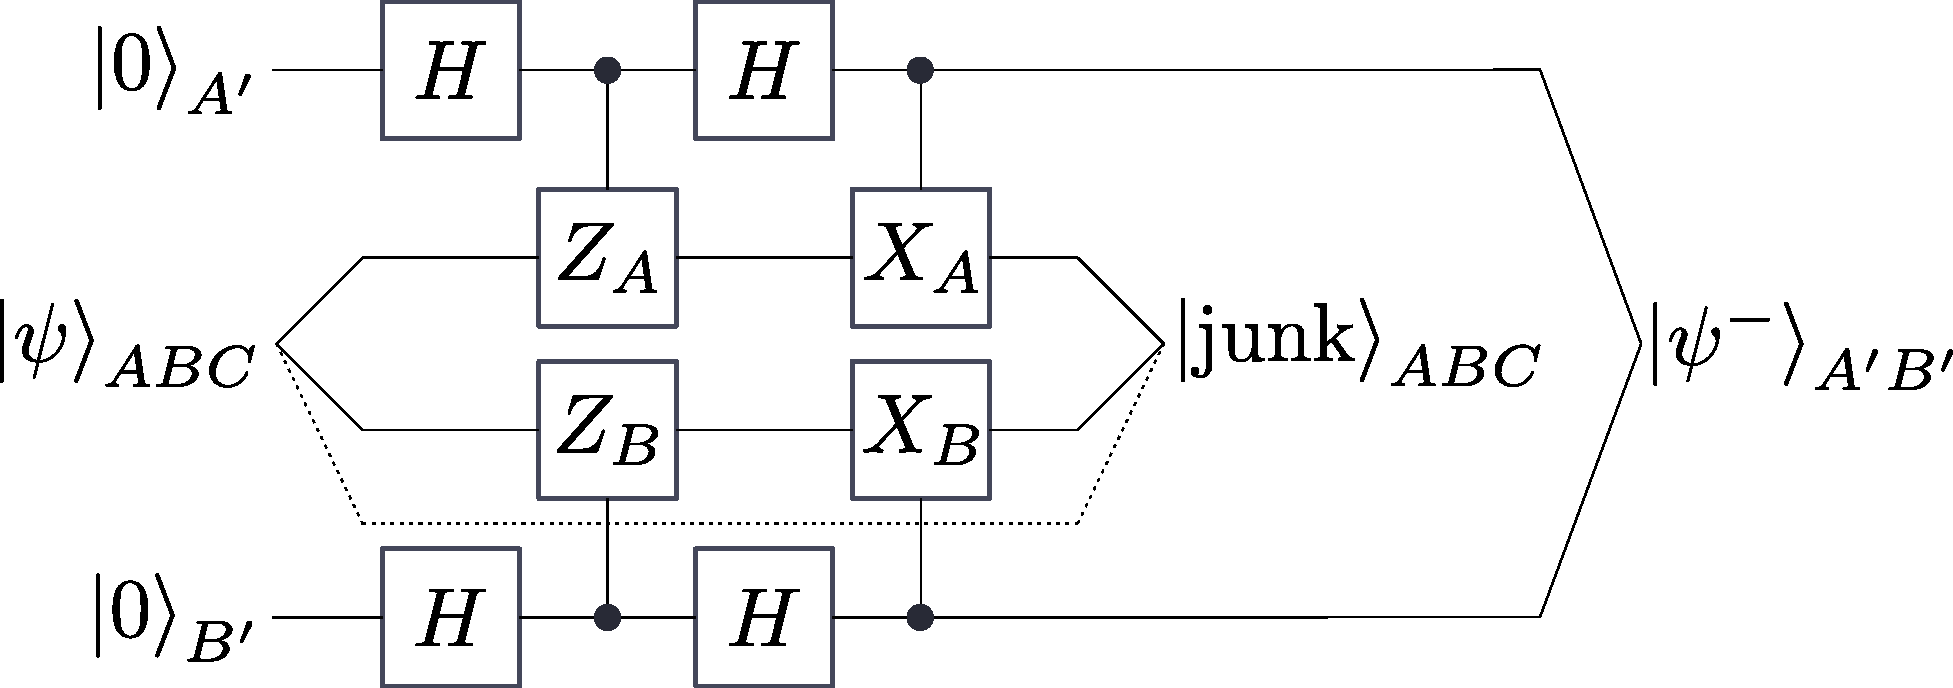
\includegraphics[width=0.95\textwidth]{chapters/selftesting/img/swap.pdf}
%	\end{center}
%	\caption{Circuit representation of the isometry $\Lambda$ extracting the target state, here $\ket{\psi^-}$, into ancillaries $A"B'$ with the correct dimesion. $H$ is the Hadamard gate, $Z$ and $X$ are control gates on the ancillaries.}
%	\label{fig:swap}
%\end{figure}
%
%Let us first build the operators $X$ and $Z$ from Alice and Bob's observables, following
%\begin{equation}
%	\begin{split}
%		Z_A = A_0, \qquad &X_A = A_1, \\
%		Z_B = \frac{B_0 - B_1}{\sqrt{2}}, \qquad &X_B = \frac{B_0 + B_1}{\sqrt{2}}. \\ 
%	\end{split}
%\end{equation}
%For $\Lambda$ to be a physical isometry, these operators have to be Hermitian and unitary.
%Since we know that $A_x,B_y$ are Hermitian, and given that the sum of Hermitian matrices are Hermitian, our operators are Hermitian.
%Trivially, $Z_A$ and $X_A$ are unitary. 
%However, this is not the case for $Z_B$ and $X_B$, we need to \textit{regularise} them.
%As detailed in \cite{Supic2019}, from an Hermitian operator $O$, we build an operator $O^\star$ by changing all the zero eigenvalues of $O$ to $1$, from which we construct a unitary operator $O'$ following $O'=|O^\star|^{-1} O^\star$.
%Thanks to \refeq{aliceBobMeasEquivalence}, we can show that $Z_B'$ and $X_B'$ act the same way as $Z_B$ and $X_B$ on any state $\ket{\psi}$ following
%\begin{equation}
%	\begin{split}
%		||(O_B' - O_B) \ket{\psi}|| &= ||(\id - O_B^\dag O_B)\psi|| \\
%									&= ||(\id-|O_B|)\ket{\psi}|| \\
%									&= ||(\id-|O_A O_B|)\ket{\psi}|| \\
%									&\leq ||(\id-O_A O_B)\ket{\psi}|| \\
%									&= 0
%	\end{split}
%\end{equation}
%where $O$ can be replaced by either $X$ or $Z$.
%
%We can now compute the effect of the isometry on the shared system and the ancillas
%\begin{equation}
%	\begin{split}
%		\Lambda[\ket{00}_{A'B'} \otimes \ket{\psi}_{ABC}] = &\frac{1}{4}\Bigg[\ket{00}_{A'B'}\otimes(\id+Z_A)(\id+Z_B)\ket{\psi}_{ABC} \\
%													   & + \ket{01}_{A'B'} \otimes X_B(\id+Z_A)(\id-Z_B)\ket{\psi}_{ABC} \\
%													   & + \ket{10}_{A'B'} \otimes X_A(\id-Z_A)(\id+Z_B)\ket{\psi}_{ABC} \\
%													   & + \ket{11}_{A'B'} \otimes X_AX_B(\id-Z_A)(\id-Z_B)\ket{\psi}_{ABC} \Bigg]
%	\end{split}	
%	\label{eq:swap_output}
%\end{equation}
%To simplify this, we first use \refeq{aliceBobMeasEquivalence} to derive the following equivalence relations
%\begin{equation}
%	X_A \ket{\psi} = X_B \ket{\psi}, \qquad Z_A \ket{\psi} = Z_B \ket{\psi}.
%	\label{eq:ABMeasEquivalence}
%\end{equation}
%In \refeq{swap_output}, replacing $Z_A$ with $Z_B$ cancels all the term of the form $(\id\pm Z_A)(\id\mp Z_B)=(\id-Z_A^2)=0$, leading to
%\begin{equation}
%	\begin{split}
%		\Lambda[\ket{00}_{A'B'} \otimes \ket{\psi}_{ABC}] = &\frac{1}{4}\Bigg[\ket{00}_{A'B'}\otimes(\id+Z_A)(\id+Z_B)\ket{\psi}_{ABC} \\
%													   & + \ket{11}_{A'B'} \otimes X_AX_B(\id-Z_A)(\id-Z_B)\ket{\psi}_{ABC} \Bigg]
%	\end{split}	
%\end{equation}
%By construction we have $\{Z_A,X_A\}=0$ and, from the anticommuting relation \refeq{anticommuting}, we have $\{Z_B,X_B\}\ket{\psi}=0$, which together with \refeq{ABMeasEquivalence} allow us to write
%\begin{equation}
%	\begin{split}
%		X_A X_B (\id - Z_A)(\id-Z_B)\ket{\psi}_{ABC} &= (\id + Z_A)(\id +Z_B)X_A X_B \ket{\psi}_{ABC}\\
%									 &= (\id + Z_A)(\id + Z_B)\ket{\psi}_{ABC} \\
%									 &= (\id + Z_A)^2\ket{\psi}_{ABC} \\
%									 &= 2(\id + Z_A)\ket{\psi}_{ABC}
%	\end{split}
%\end{equation}
%Combing these expressions, the output of the isometry $\Lambda$ is given by
%\begin{equation}
%	\Lambda[ \id_{A'B'} \otimes \ket{\psi}_{ABC} ] = \underbrace{\frac{1}{2}\left( \ket{00}_{A'B'} + \ket{11}_{A'B'} \right)}_{\ket{\phi^+}_{A'B'}} \otimes \underbrace{\frac{1+Z_A}{2}\ket{\psi}_{ABC}}_{\ket{\text{junk}}_{ABC}}
%	\label{eq:isometry}
%\end{equation}
%
%To get the self-testing statement ~\refeq{self-testing_statement}, Alice can apply an extra $\sigma_z$ gate on the $A'$ system, while Bob applies $\sigma_x$ on $B'$, transforming $\ket{\phi^+}_{A'B'}$ into $\ket{\psi^-}_{A'B'}$. These two gates can be freely embedded in $\Lambda$ as they are local unitaries on the ancillas.
%
%Note that the purification space is left untouched under $\Lambda$. This can be seen from the construction of the operator $Z_A,X_A,Z_B$ and $X_B$, and they are composed of Alice and Bob observables, not acting on $\Hil^C$. 
%
